\documentclass[mathserif,handout]{beamer}
%\documentclass{beamer}
\usetheme{metropolis}
\usepackage{amsmath,verbatim}
\usepackage{listings}
\usepackage[english]{babel}
%\usepackage{movie15}
\usepackage{multimedia}
\setbeamercovered{transparent}

\newcommand{\Deltap}{\ensuremath{\Delta^{\!+}}}
\newcommand{\trans}{\ensuremath{{}^\mathrm{T}}}
\newcommand{\eps}{\varepsilon}
\newcommand*{\approxdist}{\mathrel{\vcenter{\offinterlineskip
\vskip-.25ex\hbox{\hskip.55ex$\cdot$}\vskip-.25ex\hbox{$\sim$}
\vskip-.5ex\hbox{\hskip.55ex$\cdot$}}}}

% \lstMakeShortInline[language=myR]¬

\lstdefinelanguage{myR}
{
   language=R,
   otherkeywords={read.table, set.seed, head},
   deletekeywords={url,codes, t, dt, Call, formula,Q, R, on,by,hat,is,
col, set,start,end,deltat,zip},
   sensitive=true,
   breaklines=true,
   morecomment=[l]{\#},
   morestring=[b]",
   morestring=[b]',
   basicstyle =\ttfamily\small,
   keywordstyle=\bfseries,
   showtabs=false,
   showstringspaces=false,
   literate= {~}{$\sim$}{2},
   numberstyle=\sffamily\scriptsize,
   stepnumber=2
 }



\title{Discussion of: Unbiased MCMC with couplings (Jacob \emph{et al})}
\author{\textbf{\large Darren 
Wilkinson} \\
\url{@darrenjw}\\
\alert{\url{darrenjw.github.io}}\\
Newcastle University and The Alan Turing Institute\\}
\date{RSS, Errol Street, London\\11th December, 2019}

\begin{document}

\frame{\titlepage}

\frame{
  \frametitle{Overview}
  \begin{itemize}
\item Since in general we cannot initialise an MCMC chain with an exact sample from the target, we rely on asymptotic convergence to equilibrium, but diagnosing ``burn in'' and ``convergence'' is difficult
\item The method outlined in the read paper does not solve the ``exact sampling'' problem, but instead provides a method for removing the bias from any estimates that are produced from the algorithm output, using a pair of coupled chains
\item The approach is quite general, and can potentially be applied to many different kinds of MCMC algorithms --- this paper concentrates on MH and Gibbs sampling (so I will, too), but there are a bunch of related papers exploring applications to other MCMC schemes
  \end{itemize}
My materials: \alert{\url{https://github.com/darrenjw/unbiased-mcmc}}
}

\frame{
  \frametitle{Coupled Metropolis chains (with offset of 1)}
\centerline{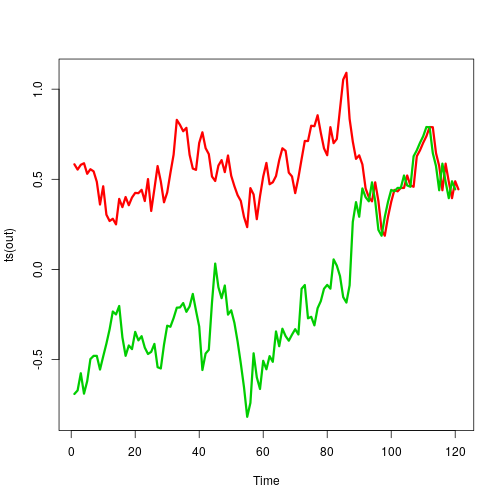
\includegraphics[height=0.95\textheight]{figs/coupled-mh}}
}

\frame{
\frametitle{Coupling versus convergence}
\begin{itemize}
\item Time-averaged estimator:
\begin{align*}
H_{k:m}(X,Y) &= \frac{1}{m-k+1}\sum_{t=k}^m h(X_t)\\
&\mbox{}\qquad +\sum_{t=k+1}^{\tau-1}\min\left(1,\frac{t-k}{m-k+1}\right)\{h(X_t)-h(Y_{t-1})\}
\\
&\equiv \text{MCMC}_{k:m} + \text{BC}_{k:m}
\end{align*}
\item
  Just the regular MCMC estimate with a correction term that terminates once the chains have coupled
\item Coupling depends on the (arbitrary) proposed coupling mechanism as well as the mixing properties of the chain
\item Possible to engineer early coupling (via initial conditions and MH kernel, for example), but this might be a dangerous strategy (see multi-modal example in paper)
\end{itemize}
}

\frame{
\frametitle{Coupling Gibbs samplers}
\begin{itemize}
\item The technique for coupling MH kernels works for multivariate as well as univariate samplers, though reflection maximal coupling works much better than a simple $\gamma$-maximal coupling in high dimensions
\item However, it also makes sense to want to couple Gibbs samplers and other component-wise update algorithms
\item For each component update of a Gibbs sampler, just couple the full-conditionals for the two chains
\item Once all components have coalesced, the full state of the chain will be coalesced, and the coupling of the two chains will be faithful
  \item Little theory providing reassurance that this will happen in reasonable time, but seems to work empirically
\end{itemize}
}
  
\frame{ 
\frametitle{Coupled Gibbs sampler for an AR(1)}
Consider an AR(1) process defined by
$$
X_t = \alpha X_{t-1} + \epsilon_t,\qquad \epsilon_t \sim N(0,\sigma^2),
$$
for $t=1,2,\ldots,N$, with periodic boundaries (so that $X_0\equiv X_N$ and $X_{N+1}\equiv X_1$), and stationary variance $\sigma^2/(1-\alpha^2)$. The full-conditional for each variable $X_t$ is of the form
$$
X_t|X_{t-1},X_{t+1} \sim N\left(\frac{\alpha}{1+\alpha^2}(X_{t-1}+X_{t+1}), \frac{\sigma^2}{1+\alpha^2} \right).
$$
We run two chains by cycling through each variable in turn and sampling from the coupled full conditionals. Here we use $N=200$ and $\alpha=0.99$, for $n=500$ iterations.
}

\frame{
  \frametitle{Coupled AR(1) chains}
\centerline{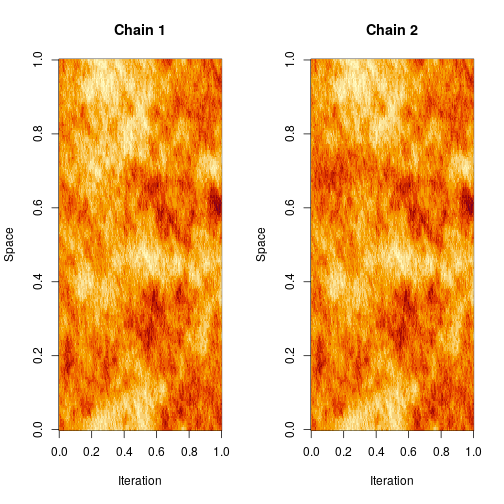
\includegraphics[height=0.95\textheight]{figs/ar1-chains}}
}

\frame{
  \frametitle{Coupled AR(1) variables}
\centerline{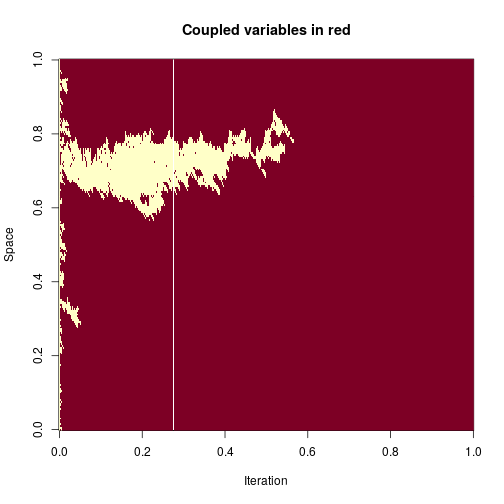
\includegraphics[height=0.95\textheight]{figs/ar1-coupled-1}}
}

\frame{
  \frametitle{Coupling behaviour for pairs of AR(1) chains}
\centerline{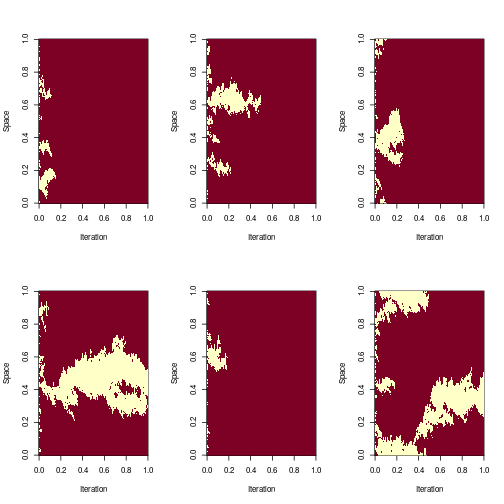
\includegraphics[height=0.95\textheight]{figs/ar1-coupled-6}}
}


\frame{
  \frametitle{Gibbs sampler for a GMRF}
  \begin{itemize}
  \item For a more challenging/interesting example, consider a Gaussian Markov random field (on a torus) with full-conditionals
    \[
X_{i,j}|\cdot \sim N\left(\frac{\alpha}{4}(X_{i-1,j}+X_{i+1,j}+X_{i,j-1}+X_{i,j+1}), \sigma^2 \right).
\]
\item Exact simulation is possible, but here we run two chains by cycling through each pixel in turn and sample from the coupled full conditionals. Here we use a $150\times 150$ grid (22.5k variables) with  $\alpha=0.99$, and $\sigma^2=1$, and run chains until they couple in order to study the coupling time distribution (for 1k replicates).
  \item Note that the coupling times become \alert{very} bad in the improper $\alpha=1$ case.
  \end{itemize}
}


\frame{
  \frametitle{Gibbs sampler for a GMRF}
    \movie{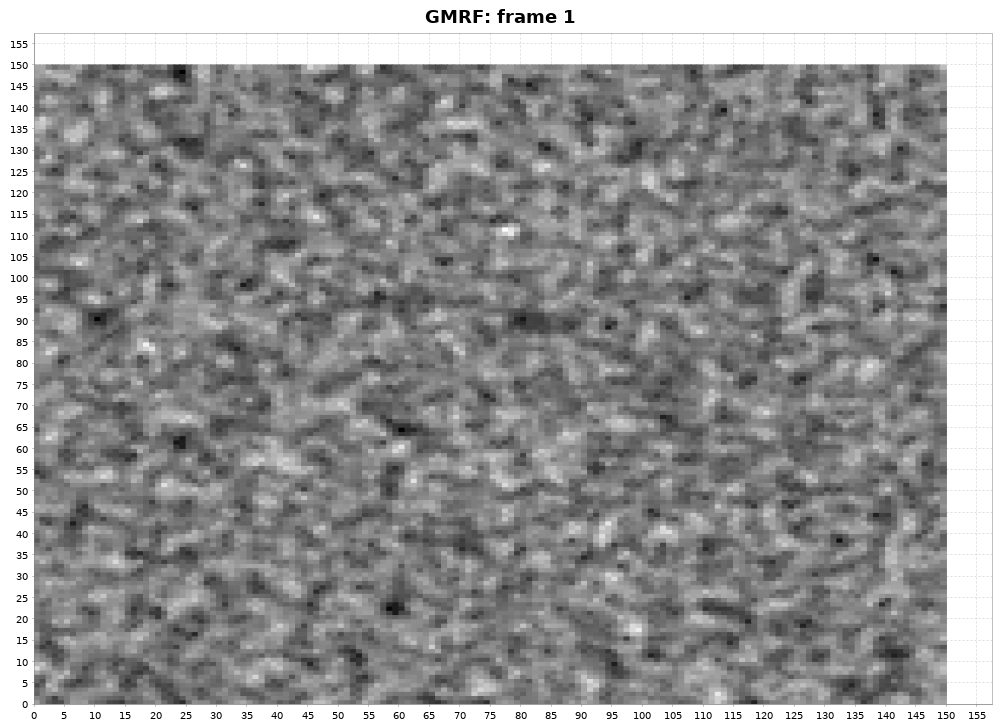
\includegraphics[height=0.85\textheight]{figs/gmrf-frame}}{gmrf-sim.mp4}
}

\frame{
  \frametitle{Coupling of pixels for a GMRF}
    \movie{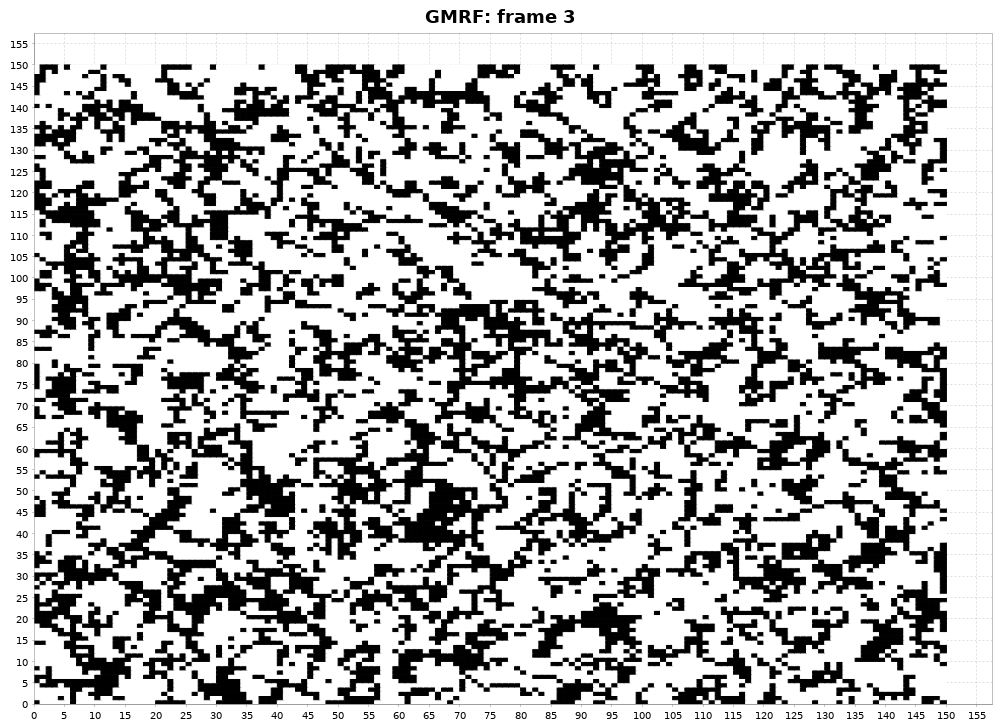
\includegraphics[height=0.85\textheight]{figs/gmrf-frame-c}}{gmrf-coupling.mp4}
}

\frame{
  \frametitle{Coupling time distribution}
\centerline{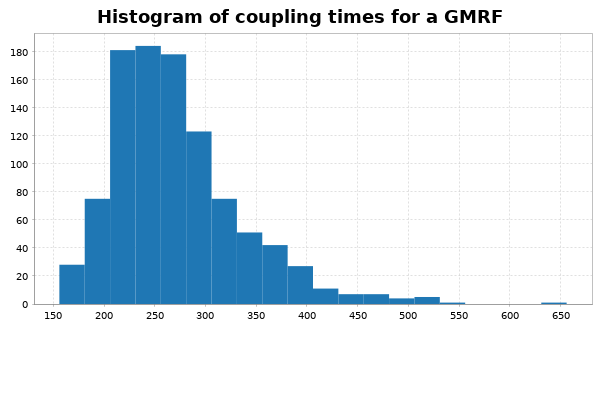
\includegraphics[height=0.5\textheight]{figs/histogram-150-gmc}
  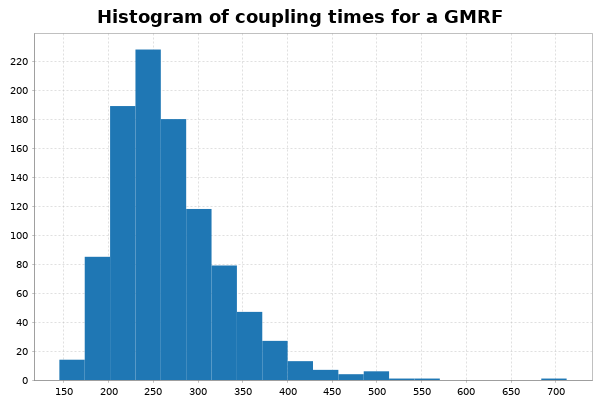
\includegraphics[height=0.4\textheight]{figs/histogram-150-rmc}}
\begin{itemize}
\item Histograms of coupling time distributions (for 1k replicates), based on $\gamma$-maximal coupling (left) and reflection maximal coupling (right)
  \item Very similar profiles, and execution times, with the reflection coupling being slightly faster in terms of CPU time
  \end{itemize}
}



\frame{
  \frametitle{Coupling time distribution}
  \begin{itemize}
    \item Using the standard \alert{maximal coupling}, the mean coupling time is around 272, and median around 260. The maximum observed coupling time is 656.
    \item Using the \alert{reflection maximal coupling}, the mean coupling time is around 268 and the median is around 257. The maximum observed coupling time is 712.
    \item This is consistent with other experiments I've done. For univariate kernels, the reflection coupling is no worse than the standard ($\gamma$) coupling, and sometimes slightly better
    \item The reflection coupling is really designed for high dimensional Gaussian kernels, where it encourages positive correlation between generated values
      \item In the univariate case, it's not immediately obvious that the reflection coupling should be better than the standard coupling
  \end{itemize}
  }

\frame{
\frametitle{Parallel chains}
\begin{itemize}
\item One of the main motivations for obtaining unbiased estimation of posterior expectations is to fix one of the issues with parallel chains MCMC
\item We would like to run many chains independently on different processors and then pool results in some way
\item In this case any bias in the chains will not ``average out'' across multiple processors, since there will be non-negligible bias in every chain
\item Unbiased estimators can be safely averaged to get new unbiased estimators with reduced variance
\item However, the debiasing doesn't actually eliminate burn-in - it just corrects for it, so you still have repeated burn-in, limiting the scalability of the parallel chains approach
\end{itemize}
}

\frame{
  \frametitle{Using coupled chains in parallel}
  \begin{itemize}
  \item The paper recommends choosing $k$ as a high quantile of the coupling time distribution, and $m$ a multiple of~$k$
  \item This is very consistent with the approach that would be taken for a (biased, uncoupled) parallel chains approach, with $k$ playing the role of ``burn-in''
  \item It might be ``dangerous'' to choose $k$ this way if early coupling has been (artificially) engineered
  \item In any case, any non-zero $k$ limits speed-up of parallel coupled chains relative to ``one long run'', via \alert{Amdahl's law} for parallel chains MCMC (Wilkinson, 2005):
    \[
\text{SpeedUp}(N) = \frac{b+n}{b+\frac{n}{N}} \overset{N}{\underset{\infty}{\longrightarrow}} \frac{b+n}{b},
    \]
    for burn-in $b$ and monitoring run $n$ on $N$ processors (eg. asymptotic limit of 10 for $n=9b$).
    \end{itemize}
}

\frame{
  \frametitle{Conclusion}
  \begin{itemize}
  \item The method proposed in the paper is often straightforward to implement, and seems to work well on a range of problems
  \item It is potentially useful in the context of parallelisation of MCMC algorithms, since averaging unbiased estimators is relatively ``safe'', but it is not clear that it fundamentally solves the ``parallel MCMC'' problem, since some kind of ``burn-in'' must still be repeated for every pair of chains
  \item Many open questions regarding the co-development of MCMC and coupling algorithms for overall efficiency
  \item Overall, an interesting and discussable contribution to the literature, so \alert{it gives me great pleasure to propose the vote of thanks!}
  \end{itemize}
My materials: \alert{\url{https://github.com/darrenjw/unbiased-mcmc}}
}


\end{document}
